\documentclass[11pt]{article}

\usepackage[margin=1in]{geometry}
\usepackage{graphicx}
\usepackage{subcaption}
\usepackage{amsmath}
\usepackage{amssymb}
\usepackage{float}

\title{RL Lab 5 - Value Function Approximation and Control}
\author{Adonis Jamal}
\date{}

\begin{document}
\maketitle

\section{SARSA Agent}
\subsection{Please upload the graph corresponding to the evolution of the average number of steps per episode throughout the training. Comment on the graph.}
\begin{figure}[H]
    \centering
    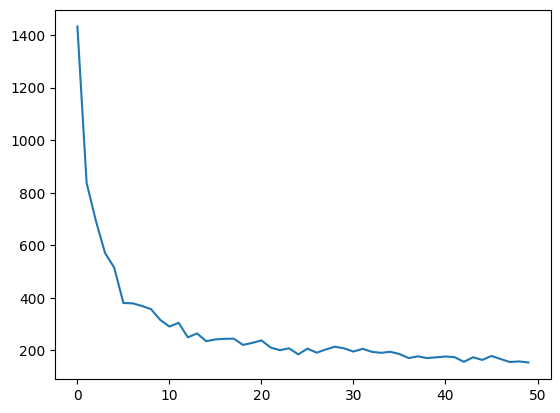
\includegraphics[width=0.8\textwidth]{figures/average_steps_per_episode.png}
    \caption{Average number of steps per episode over 50 episodes, averaged across 10 independent runs.}
\end{figure}

The graph depicts the average number of steps per episode over 50 episodes averaged across 10 independent runs. At first, the average number of steps per episode is high, as the agent is exploring and learning about the environment. As the agent learns, the average number of steps per episode decreases sharply, up to around episode 10, which indicates that the agent quickly identifies a good and efficient policy for reaching the goal. After this initial learning phase, the average number of steps per episode continues to decrease, but at a much slower rate, indicating that the agent is fine-tuning its policy and entering a phase of diminishing returns. After that, only small oscillations are observed, which suggests that the agent has converged to a near-optimal policy and is consistently performing well in the environment. Due to the stochastic nature of the environment and the learning process, notably the continued $\epsilon$-greedy exploration, the average number of steps per episode does not stabilize completely, but the overall trend indicates that the agent has successfully learned to navigate the environment efficiently.


\subsection{Comment on the graph showing the influence of the tiles' configuration on the agent's learning and interpret the results. Please attach the corresponding graph to your answer.}
\begin{figure}[H]
    \centering
    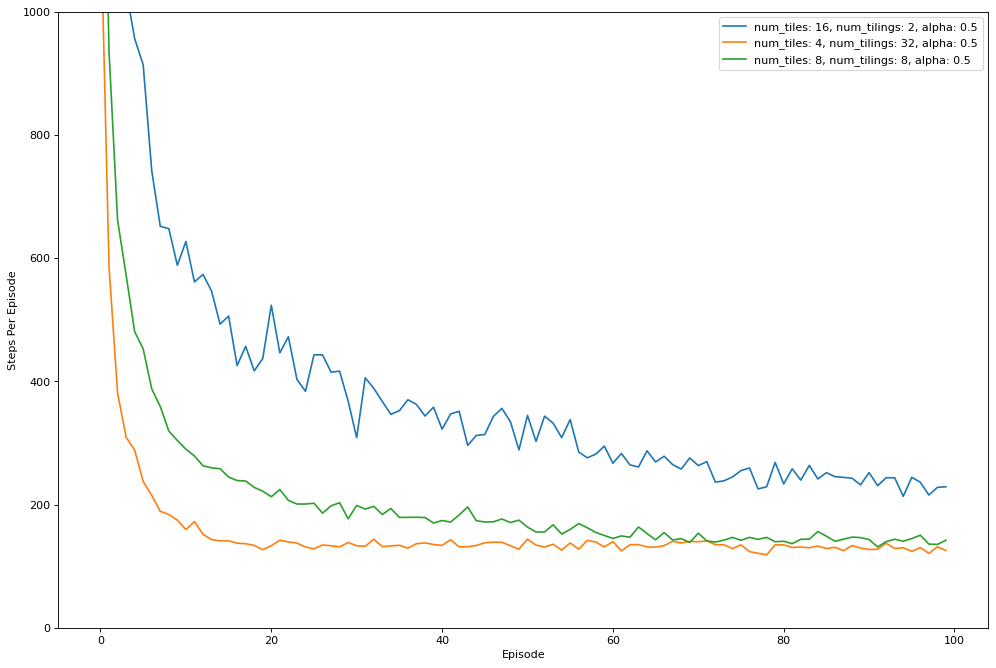
\includegraphics[width=0.8\textwidth]{figures/average_steps_per_episode_tile_config.png}
    \caption{Average number of steps per episode for different tile configurations, averaged across 20 independent runs.}
\end{figure}

The results indicate that the way the 512 features are arranged is more important than the total number of features. The setting with 32 tilings of $4 \times 4$ tiles learns the most efficiently, with a rapid reduction in the average number of steps during the first part of training. This behavior suggests that the high degree of overlap between the tilings allows the agent to generalize more effectively across similar states, allowing it to transfer learning from one state to another more efficiently. The 8 tilings of $8 \times 8$ tiles also improves steadily and reaches a comparable level, but its progress is slightly slower at the beginning, which is consistent with a more balanced but less redundant representation. In contrast, the 2 tilings of $16 \times 16$ tiles produces the weakest learning curve, with higher step counts throughout training. Although the tiles are finer, the very small number of tilings limits feature overlap and therefore reduces the agent's ability to generalize from limited experience. The comparison suggests that having more tilings with coarser tiles leads to better learning performance than having fewer tilings with finer tiles, even when the total number of features is the same.

\end{document}
